\documentclass[11pt,letterpaper]{article}
\usepackage[margin=0.6in]{geometry}
\usepackage{amsmath,amssymb}
\usepackage{tikz}
\usetikzlibrary{arrows.meta,positioning}
\usepackage{xcolor}
\usepackage{fontawesome5}
\usepackage{tcolorbox}
\usepackage{multicol}
\usepackage{enumitem}
\usepackage{hyperref}

\definecolor{primaryblue}{RGB}{41, 98, 255}
\definecolor{accentgreen}{RGB}{0, 150, 136}
\definecolor{warnorange}{RGB}{255, 152, 0}
\definecolor{lightgray}{RGB}{245, 245, 245}

\tcbset{
    conceptbox/.style={colback=primaryblue!5, colframe=primaryblue, boxrule=1pt, arc=3pt, left=5pt, right=5pt, top=5pt, bottom=5pt},
    formulabox/.style={colback=lightgray, colframe=gray!50, boxrule=0.5pt, arc=2pt, left=5pt, right=5pt, top=3pt, bottom=3pt},
    warningbox/.style={colback=warnorange!10, colframe=warnorange, boxrule=1pt, arc=3pt, left=5pt, right=5pt, top=5pt, bottom=5pt},
    appbox/.style={colback=accentgreen!5, colframe=accentgreen, boxrule=1pt, arc=3pt, left=5pt, right=5pt, top=5pt, bottom=5pt}
}

\pagestyle{empty}
\setlength{\parindent}{0pt}
\setlist[itemize]{leftmargin=*, itemsep=1pt, topsep=2pt}

\begin{document}

\begin{center}
{\LARGE\bfseries\color{primaryblue} Chapter 7: Vector Spaces}\\[3pt]
{\large Basis, Projections, and Linear Transformations}
\end{center}
\vspace{-5pt}
\hrule height 2pt
\vspace{8pt}

\begin{multicols}{2}

\begin{tcolorbox}[conceptbox, title={\faLightbulb\ Key Concepts}]
\begin{itemize}
    \item \textbf{Basis}: Minimal spanning set for a space
    \item \textbf{Dimension}: Number of vectors in any basis
    \item \textbf{Null Space}: Vectors mapped to zero by $A$
    \item \textbf{Range}: All possible outputs of $A$
    \item \textbf{Projection}: Closest point in a subspace
    \item \textbf{Orthogonality}: $\mathbf{u} \cdot \mathbf{v} = 0$
\end{itemize}
\end{tcolorbox}

\begin{tcolorbox}[formulabox, title={\faCalculator\ Core Formulas}]
\textbf{Projection onto vector:}
\[ \text{proj}_{\mathbf{u}}(\mathbf{v}) = \frac{\mathbf{v} \cdot \mathbf{u}}{\mathbf{u} \cdot \mathbf{u}} \mathbf{u} \]

\textbf{Projection matrix:}
\[ P = A(A^T A)^{-1} A^T \]

\textbf{Rank-Nullity Theorem:}
\[ \dim(\text{null}(A)) + \dim(\text{range}(A)) = n \]

\textbf{Least Squares Solution:}
\[ \hat{\mathbf{x}} = (A^T A)^{-1} A^T \mathbf{b} \]
\end{tcolorbox}

\columnbreak

\begin{center}
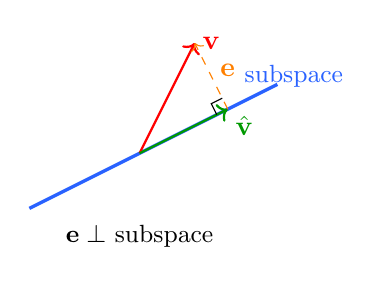
\begin{tikzpicture}[scale=0.7]
    % Subspace (line)
    \draw[primaryblue, very thick] (-2,-1) -- (2.5,1.25);
    \node[primaryblue] at (2.8,1.4) {\small subspace};

    % Original vector
    \draw[->,thick,red] (0,0) -- (1,2);
    \node[red] at (1.3,2) {$\mathbf{v}$};

    % Projection
    \draw[->,thick,green!60!black] (0,0) -- (1.6,0.8);
    \node[green!60!black] at (1.9,0.5) {$\hat{\mathbf{v}}$};

    % Error vector
    \draw[->,dashed,orange] (1.6,0.8) -- (1,2);
    \node[orange] at (1.6,1.5) {$\mathbf{e}$};

    % Right angle
    \draw (1.4,0.7) -- (1.3,0.9) -- (1.5,1);

    \node at (0,-1.5) {\small $\mathbf{e} \perp$ subspace};
\end{tikzpicture}
\end{center}

\begin{tcolorbox}[appbox, title={\faRobot\ ML Applications}]
\begin{itemize}
    \item \textbf{Word Embeddings}: Words as vectors, analogies as arithmetic
    \item \textbf{Attention}: Projection onto query/key subspaces
    \item \textbf{Linear Regression}: Least squares = projection
    \item \textbf{LoRA}: Low-rank updates in learned subspace
    \item \textbf{Orthogonal Init}: Better gradient flow
\end{itemize}
\end{tcolorbox}

\begin{tcolorbox}[warningbox, title={\faExclamationTriangle\ Common Pitfalls}]
\begin{itemize}
    \item Projection is \textbf{idempotent}: $P^2 = P$
    \item Gram-Schmidt can be \textbf{numerically unstable}
    \item $A^T A$ can be singular --- use pseudoinverse
    \item Don't confuse row space with column space
\end{itemize}
\end{tcolorbox}

\end{multicols}

\vspace{5pt}
\hrule
\vspace{5pt}

\begin{center}
\faGithub\ \textbf{Notebook}: \url{https://github.com/vijaygwu/math-powers-ai/blob/main/notebooks/ch07_vector_spaces.ipynb}
\end{center}

\end{document}
